\appendix

\chapter{Ancillary explanations of algorithms and concepts}

\section{Discretisation}
Grid-based graph: $d_{G}(L_{O},M) \rightarrow G_{M,G}$\\
\noindent
An octile lattice $L_{N,O}$ is laid over $M$ such that each node in $L_{N,O}$ lies directly on top of a coordinate $(x,y)$ in $M$. If none of the (up to) four cells surrounding a node are free then that node is removed,\footnote{In a map $M$ of size $N^{2}$, the ``four cells surrounding'' a node that represents coordinate $(a,b) \in M$ are the cells $(a,b)$, $(a,b-1)$, $(a-1,b-1)$ and $(a-1,b)$ if they exist, where $0 \leq a,b \leq N$.} along with all edges that are connected to it. Additionally, if a cell is blocked, diagonal edges that cross that cell are removed, along with any horizontal or vertical edges that lie beneath the blocked cell and are also on the boundary of the lattice.\\

\noindent
Visibility graph: $d_{V}(L_{O},M) \rightarrow G_{M,V}$\\
\noindent
A full lattice $L_{N,O}$ is laid over $M$ such that each node in $L_{N,O}$ lies directly on top of a coordinate $(x,y)$ in $M$. Unless {\em either} exactly three of the (up to) four cells surrounding a node are free {\em or} the node is $n_{start}$ or $n_{goal}$ then that node is removed, along with all edges that are connected to it --- since such nodes are guaranteed to not be on the shortest path. In addition each edge $(n,n') \in E$ is removed if there is no line of sight between the locations that $n$ and $n'$ represent.\\

\section{A* with post-smoothing}
This section is in reference to the pseudo-code in Algorithm 3:\\

\noindent On each iteration, the algorithm considers a node $n_{curr}$. Starting with $n_{curr} = n_{goal}$ a line of sight test is performed from the location represented by $n_{curr}$ to the location represented by $n_{curr}.parent.parent$ (line 6). If a line of sight exists, $n_{curr}.parent$ is set to $n_{curr}.parent.parent$ (line 7) --- this has the effect of adding an edge $(n_{curr},n_{curr}.parent.parent)$ to $G$. This process is repeated on $n_{curr}$ until a line of sight test fails, at which point $n_{curr}$ is set to $n_{curr}.parent.parent$ (line 14, and note that $n_{curr}.parent.parent$ is the node on which the line of sight test failed), and the next iteration commences. When $n = n_{start}$, the algorithm terminates (lines 12-13).\\

\section{Theta*}
This section is in reference to the pseudo-code in Algorithm 4:\\

\noindent If a line of sight exists between $n_{neigh}.coord$ and $n_{curr}.parent.coord$ (line 1), {\em Theta*} (notionally) creates an edge $e = (n_{neigh}, n_{curr}.parent) \in G$ and attempts to relax $e$ (lines 2-5). However, if the line of sight does not exist $e$ is removed from $G$ and {\em Theta*} mimics {\em A*} by attempting to relax the edge $(n_{neigh},n_{curr})$, as per the {\tt Update} subroutine of {\em A*} (lines 10-13).


\section{Lazy Theta*}
This section is in reference to the pseudo-code in Algorithm 5:\\

\noindent For each $n_{curr}$ that is expanded, {\em Lazy Theta*} assumes that a line of sight exists between $n_{curr}.parent$ and each neighbour $n_{neigh}$ of $n_{curr}$, and updates the {\em g-value} and $parent$ of each $n_{neigh}$ accordingly (i.e. {\em Lazy Theta*} performs the update part of relaxation without first performing the test in equation (2.1), lines 21-24). {\em Lazy Theta*} only actually performs that line of sight test if the $n_{neigh}$ itself is ever expanded (i.e. now the new $n_{curr}$), by calling {\tt Initialise} when $n_{curr}$ is popped off $openSet$. If the line of sight does not in fact exist, {\tt Initialise} alters $n_{curr}$ accordingly (lines 17-20).

\section{Line of Sight algorithm}
This section is in reference to the pseudo-code in Algorithm 8:\\

\noindent
As stated in 3.2.4, the {\em Line of Sight} algorithm is based on the pseudo-code in the publication of the {\em Theta*} algorithm \cite{Daniel10},\footnote{I have re-named the value $f$ that is used in the {\em Line of Sight} algorithm in the publication of the {\em Theta*} algorithm as $s$, to avoid confusion with the $f-value$ of a node that is used elsewhere in this dissertation.} which itself is a derivative of {\em Bresenham's line drawing algorithm}\cite{Bresenham65}.\\

\noindent
For the purposes of clarity, the pseudocode presented in Algorithm 8 assumes that the straight line between locations $a$ and $b$ is in `octant 1' - i.e. the angle that the line $ab$ makes with the horizontal is between $0^{o}$ and $45^{o}$.\\

\noindent
The key variables of the algorithm are:
\begin{description}
\item{$i$ and $j$} --- integers that represent the coordinate of the cell being considered. The algorithm only considers cells that the line $ab$ passes through.
\item{$s$} --- a value that represents the point at which the line $ab$ intersects $i+1$, with respect to the current $j$ value, i.e. when the algorithm is considering cell $(i,j)$ while doing a line of sight test between location $a$ at $(i_{a},j_{a})$ and location $b$ at $(i_{b},j_{b})$, $s = (y(i+1)/j)\Delta i$, where $y(i+1)$ is the y-coordinate of the point at which the line $ab$ intersects $i+1$, and $\Delta i = i_{b} - i_{a}$. The $s$ value determines how many cells in column $i$ above the current cell ($(i,j)$ will be checked.
\end{description}

\noindent{\bfseries Algorithm} - assuming octant 1\\
\noindent
The algorithm starts by considering the cell with coordinate $a$. If every cell in column $i_{a}$ that the line $ab$ passes through is free, then column $i_{a+1}$ is considered, and so on. If column $i_{b}$ is reached without any blocked cells detected, the algorithm returns {\em true}, otherwise it returns {\em false}.\\

\noindent
$s$ determines which cells the algorithm needs to check to find out whether they are blocked:
\begin{itemize}
\item $s > \Delta i$ indicates that the line $ab$ intersects $i+1$ somewhere above cell $(i,j)$ --- so the algorithm checks whether $(i,j)$ is blocked. If it is then the algorithm returns $false$ but if it isn't then $j$ is increased so that the next cell to be considered is $(i+1,j)$ (see Figure A.1, cell $(0,0)$).
\item $0 < s \leq \Delta i$ indicates that the line $ab$ intersects $i+1$ in the cell currently being considered --- so the algorithm checks whether $(i,j)$ is blocked. If it is then the algorithm returns $false$ but if it isn't then $i$ is increased so that the next cell to be considered is $(i+1,j)$ (see Figure A.1, cell $(1,0)$).
\item $s = 0 \land \Delta j \neq 0$ indicates that the line $ab$ is intersects $i+1$ at exactly $j+1$ --- so the algorithm does not need to check whether $(i,j)$ is blocked, because of the zero-width agent assumption made in subsection 2.1.1. Therefore, $i$ and $j$ are increased so that the next cell to be considered is $(i+1,j+1)$ (see Figure A.1, cell $(2,2)$).
\item $s = 0 \land \Delta j = 0$ indicates that the line $ab$ is horizontal --- so the algorithm checks whether $(i,j)$ and $(i,j-1)$ are blocked. If it is then the algorithm returns $false$ but if it isn't then $i$ is increased so that the next cell to be considered is $(i+1,j)$.\footnote{To avoid the possibility of the final clause in the condition throwing an {\tt ArrayIndexOutOfBoundsException}, an extra $x$-coordinate check or a {\tt try-catch} block would also be required.} This case is not illustrated in Figure A.1.
\end{itemize}

\begin{figure}
\centering
  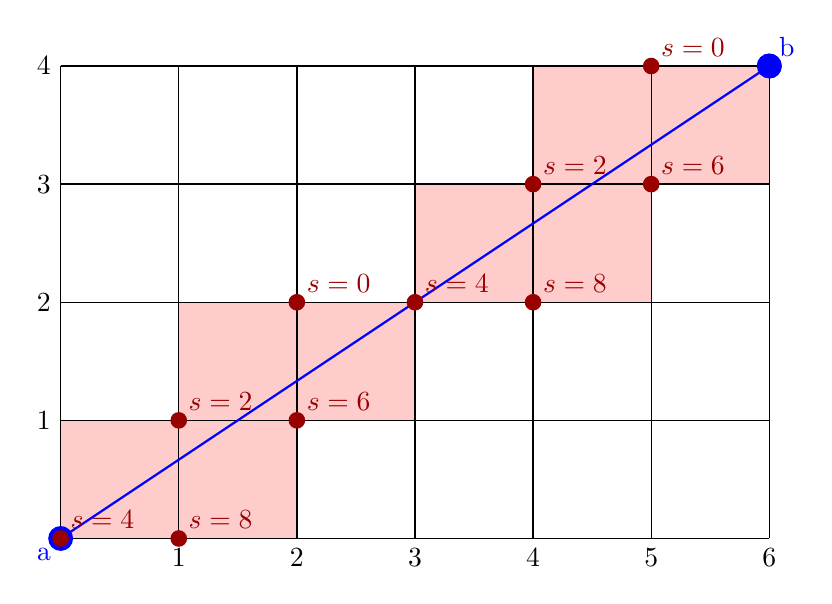
\begin{tikzpicture}[scale=1.5,line width=0.5pt]
    \draw (0,0) grid (6,4);

    \node[below left, blue] at (0,0) {a};
    \node[below] at (1,0) {1};
    \node[below] at (2,0) {2};
    \node[below] at (3,0) {3};
    \node[below] at (4,0) {4};
    \node[below] at (5,0) {5};
    \node[below] at (6,0) {6};

    \node[left] at (0,1) {1};
    \node[left] at (0,2) {2};
    \node[left] at (0,3) {3};
    \node[left] at (0,4) {4};
    \node[above right, blue] at (6,4) {b};
    \fill[blue] (6,4) circle (3pt);

    \filldraw[color=black,fill=red!20] (0,0) rectangle (1,1); 
    \filldraw[color=black,fill=red!20] (1,0) rectangle (2,1);
    \filldraw[color=black,fill=red!20] (1,1) rectangle (2,2);
    \filldraw[color=black,fill=red!20] (2,1) rectangle (3,2);
    \filldraw[color=black,fill=red!20] (3,2) rectangle (4,3); 
    \filldraw[color=black,fill=red!20] (4,2) rectangle (5,3);
    \filldraw[color=black,fill=red!20] (4,3) rectangle (5,4);
    \filldraw[color=black,fill=red!20] (5,3) rectangle (6,4);
    
    \draw[blue, thick] (0,0) -- (6,4);
    \fill[blue] (0,0) circle (3pt);
    \fill[blue] (6,4) circle (3pt);
  
    \node[above right,red!60!black] at (0,0) {$s=4$}; \fill[red!60!black] (0,0) circle (2pt);
    \node[above right,red!60!black] at (1,0) {$s=8$}; \fill[red!60!black] (1,0) circle (2pt);
    \node[above right,red!60!black] at (1,1) {$s=2$}; \fill[red!60!black] (1,1) circle (2pt);
    \node[above right,red!60!black] at (2,1) {$s=6$}; \fill[red!60!black] (2,1) circle (2pt);
    \node[above right,red!60!black] at (2,2) {$s=0$}; \fill[red!60!black] (2,2) circle (2pt);
    \node[above right,red!60!black] at (3,2) {$s=4$}; \fill[red!60!black] (3,2) circle (2pt);
    \node[above right,red!60!black] at (4,2) {$s=8$}; \fill[red!60!black] (4,2) circle (2pt);
    \node[above right,red!60!black] at (4,3) {$s=2$}; \fill[red!60!black] (4,3) circle (2pt);
    \node[above right,red!60!black] at (5,3) {$s=6$}; \fill[red!60!black] (5,3) circle (2pt);
    \node[above right,red!60!black] at (5,4) {$s=0$}; \fill[red!60!black] (5,4) circle (2pt);

  \end{tikzpicture}
  \caption[Line of Sight algorithm]{Cells checked by the Line of Sight algorithm, where $\Delta i = 6$ and $\Delta j = 4$} 
\end{figure}

\section{Query to a bitwise-and-geometrically compressed $LDDB_{N}$}

Figure 3.11 gives an annotated explanation of a query to a bitwise-and-geometrically compressed $LDDB$ using a block size of $3 \times 3$. The steps are elaborated below:

\begin{description}
\item(a) the original query requests the intermediate coordinates on the shortest path between \\ an $ingress$ of $(2,0)$ and an $egress$ of $(3,3)$ on the map shown, i.e. a map of size $3 \times 3$ \\ with integer code 48;
    
\item (b) the integer codes are calculated for all four rotations of the map, and the smallest code \\ is used for the query. The $ingress$ and $egress$ are rotated accordingly;
    
\item (c) the $y-value$ of the rotated $ingress$ coordinate is larger than that of the rotated $egress$ \\ coordinate. Therefore, the $ingress$ and $egress$ are exchanged (i.e. reflected) for the query;
    
\item (d) the final configuration for the query has been reached: map code 18 and \\ $ingress-egress$ coordinates $(3,0)-(0,1)$ which is encoded as $011-000-000-001$;
    
\item (e) the query returns a 64 bit integer, whose 32 most significant bits can be decoded as a {\tt float} \\ giving the length of the shortest path between $ingress$ and $egress$, and whose 24 least significant \\ bits are $010-010-001-010$ which is decoded as $i_{1}=(2,2)$ and $i_{2}=(1,2)$;
    
\item (f) since the coordinates were reflected in step (c), the reflection is undone in step (f). Therefore \\ the first intermediate coordinate $i_{1}=(1,2)$ and the second $i_{2}=(2,2)$;
    
\item (g) since the map was rotated 90$^{\circ}$ clockwise in step (b), the rotation is undone in step (g). \\ Therefore $i_{1}=(1,1)$ and $i_{2}=(1,2)$;
    
\item (h) the result is ready to be returned, which provides {\em Block A*} with the shortest path between \\ the $ingress$ and the $egress$, as shown.
\end{description}

\chapter{Project Proposal}

\vfil

\centerline{\Large \bf Project Proposal}
\vspace{0.4in}
\centerline{\Large A Comparison of Any-Angle Pathfinding Algorithms for Virtual Agents }
\vspace{0.4in}
\centerline{\large O. Freeman, Clare College}
\vspace{0.3in}
\centerline{\large 25$^{th}$ October 2013}
\vspace{0.3in}
\vfil

\noindent
{\bf Project Originator:} O. Freeman
\vspace{0.2in}

\noindent
{\bf Project Supervisor:} Dr. R. J. Gibbens
\vspace{0.2in}

\noindent
{\bf Director of Studies:} Prof. L. J. Paulson
\vspace{0.2in}
\noindent
 
\noindent
{\bf Project Overseers:} Dr.~S.~Clark \& Dr~P.~Li\`o


% Main document

\section*{Introduction}


Finding short and realistic-looking paths through environments with arbitrarily placed obstacles is one of the central problems in artificial intelligence for games and robotics. \\

\noindent
The environment must first be discretised into a graph so that it can be searched. Common discretisation strategies include representing the environment as a grid of blocked and unblocked cells, visibility graphs and navigation meshes. Many algorithms exist to efficiently find optimal paths through graphs, but due to its optimality and efficiency, A* is often the best choice {\em (Nash: 2012)}. However, the paths that A* produces are constrained to travel along the edges of the graph -- in a grid graph, for example, the agent is restricted to travelling at integer multiples of 45$^\circ$. Many discretisation strategies thus produce paths which are longer and have more turns than is necessary, and hence look unnatural to the human eye -- a property that is undesirable when mimicking human behaviour with robots or virtual agents.\\

\noindent
A variety of A*-inspired `any-angle' pathfinding algorithms have been proposed to solve this problem. These include:
\begin{itemize}
\item {\em Post-processing smoothing step to A* (Millington: 2009)} -- collapses multiple straight line segments using a line-of-sight algorithm.
\item {\em Field D* (Ferguson, Stentz: 2006)} -- avoids the constraint of having to travel only to existing nodes by interpolating between g-values to produce new nodes at semi-arbitrary positions.
\item {\em Theta* (Nash, Koenig: 2007)} -- allows nodes to change their parent to certain nodes within line-of-sight.  
\item {\em Block A* (Yap: 2011)} -- performs search on  $N \times N$ cell blocks whose internal optimal paths have been pre-calculated.
\end{itemize}

\noindent
The aim of this project is to compare and contrast the performance of a selection of any-angle pathfinding algorithms. The test suite will consist of randomly generated maps of differing coverage, clustering and grid resolution to ensure that the analysis of the algorithms' properties is suitable for a wide range of application domains.

\vfil

\section*{Starting Point}

My current algorithmic knowledge for this project is:

\begin{itemize}
\item {\em Part 1B CST Artificial Intelligence I} -- A* search.
\item {\em Artificial Intelligence for Games (Millington, Funge)} -- A* pathfinding. 
\end{itemize}

My current programming experience is:

\begin{itemize}
\item {\em Part 1A CST Programming in Java.}
\item {\em Part 1B CST Further Java} and {\em Group Project.}
\item {\em Internship at NaturalMotion Inc.} -– Developed a prototype GUI in Java.
\end{itemize}

\section*{Work to be done}

In order to test and compare the any-angle pathfinding algorithms, I will need to develop an application to generate maps and to run and record the performance of the algorithms. I will also need to use statistical software to evaluate the performance of the algorithms.\\ \\ The project breaks down into the following main sections:


\begin{description}
  \item[Map generation] \hfill \\
  I will develop a tool that can automatically generate maps with adjustable coverage, clustering and resolution. This may require a custom algorithm. The tool will also convert the maps into a search graph.
  \item[Testing simulator] \hfill \\
  I will develop an application that allows me to run one of a collection of algorithms on one of a collection of maps, and then visually display the resulting path and statistics about the path. Therefore the underlying framework must be modular, to allow different maps and algorithms to be used interchangeably.
  \item[Algorithm implementation] \hfill \\
  I will research and implement the any-angle path-finding algorithms.
  \item[Evaluation] \hfill \\
  I will evaluate the performance of the algorithms according to metrics such as:
  
  {\em Path} -- Path length and path straightness. \\
  {\em Graph} -- Clustering, coverage and resolution.\\
  {\em Computation} -- Execution time.
  
\end{description}

\section*{Success Criteria for the Main Result}

The following core components should be produced to declare the project a \\success:

\begin{enumerate}
\item A generator of maps of varying coverage, clustering and resolution.
\item A simulator that can:
\begin{itemize}
\item load one of a collection of maps from the generator;
\item run one of a collection of any-angle path-finding algorithms on the map and display the result visually;
\item return statistics about the performance of the algorithm on the map.
\end{itemize}
\end{enumerate}

\section*{Possible Extensions}

\begin{enumerate}
\item Extend investigation from grid-based map discretization to visibility graphs.

\item Implement a map editor that allows the user to create a custom map by selecting grid locations to be blocked.

\item Adapt the implementation and analyse the performance of the algorithms when the obstacles become traversable with high cost function -- i.e. the agent can climb over the obstacle, but only slowly.

\end{enumerate}

\section*{Resources Required and Backup Strategy}

For this project I shall mainly use my own Macbook Air (1.3GHz dual-core Intel, 4GB RAM, 128GB Disk), with backup provided on cloud storage and version control provided by GitHub. If my computer fails, I will be able to recover my work from the cloud storage and continue my project on the MCS machines.

\vfil

\section*{Timetable: Workplan and Milestones}
Project start date: 28/10/2013.\\

\begin{description}

\item[28$^{th}$ October -- 3$^{rd}$ November (1 week)] \hfill \\

{\em Project set up and familiarization}
\begin{itemize}
\item Start project note book.
\item Set up programming environment, including testing framework.
\item Set up backup strategy.
\end{itemize}
{\em Milestone}: Comfortable with development environment.\\

\item[4$^{th}$ November -- 17$^{th}$ November (2 weeks)] \hfill \\

{\em Literature research and implementation planning}
\begin{itemize}
\item Research and choose any-angle pathfinding algorithms.
\item Research and choose data structures and algorithms that will be necessary for the map generator and algorithm simulator applications.
\item Decide key interfaces of the map generator and algorithm simulator applications.
\end{itemize}
{\em Milestone}: Any-path algorithms chosen and thoroughly understood. Defining features of application identified.\\

\item[18$^{th}$ November -- 15$^{th}$ December (4 weeks)] \hfill \\

{\em Application development phase 1}
\begin{itemize}
\item Devise architecture and class structure, including any design patterns to be used.
\item Implement a prototype simulation application that renders a \\placeholder map and runs a placeholder algorithm. 
\end{itemize}
{\em Milestone}: A working prototype implementation of the simulation application.\\

\item[16$^{th}$ December -- 5$^{th}$ January (3 weeks)] \hfill \\

{\em Application development phase 2}
\begin{itemize}
\item Implement path visualisation in the application.
\item Implement statistical measurement and feedback in the application.
\end{itemize}
{\em Milestone}: Application correctly displays path and path statistics.\\

\item[6$^{th}$ January -- 26$^{th}$ January (3 weeks)] \hfill \\

{\em Path-finding algorithm implementation}
\begin{itemize}
\item Implement and test the chosen any-angle path-finding algorithms.
\end{itemize}
{\em Milestone}: Path-finding algorithms run correctly.\\

\item[27$^{th}$ January -- 9$^{th}$ February (2 weeks)] \hfill \\

{\em Map-generation algorithm implementation}
\begin{itemize}
\item Implement and test the map-generation algorithm.  
\item Test and debug the simulation application.
\end{itemize}
{\em Milestone}: Maps generated according to the input parameters.\\

\item[10$^{th}$ February -- 23$^{rd}$ February (2 weeks)] \hfill \\

{\em Progress report}
\begin{itemize}
\item Write the progress report.  
\item Prepare the presentation.
\item Start gathering data for evaluation.
\end{itemize}
{\em Milestone}: Progress report and presentation complete.\\

\item[24$^{th}$ February -- 9$^{th}$ March (2 weeks)] \hfill \\

{\em Catchup and extension}
\begin{itemize}
\item Learn R - statistical analysis software.
\item Complete any unfinished tasks. 
\item {\em Optional extension 1}: Visibility graph.
\item {\em Optional extension 2}: Custom maps.
\item {\em Optional extension 3}: Traversable obstacles.
\end{itemize}
{\em Milestone}: Code completion.\\

\item[10$^{th}$ March -- 23$^{rd}$ March (2 weeks)] \hfill \\

{\em Dissertation phase 1}
\begin{itemize}
\item Plan the structure of the Dissertation. 
\item Improve \LaTeX\ skills.
\item Write the Preparation chapter.
\item Write the Implementation chapter.
\end{itemize}
{\em Milestone}: Preparation and Implementation chapters complete.\\

\item[24$^{th}$ March -- 13$^{th}$ April (3 weeks)] \hfill \\

{\em Dissertation phase 2}
\begin{itemize}
\item Generate statistics and diagrams.
\item Write the Evaluation chapter.
\end{itemize}
{\em Milestone}: Evaluation chapter complete.\\

\item[14$^{th}$ April -- 27$^{th}$ April (2 weeks)] \hfill \\

{\em Dissertation phase 3}
\begin{itemize}
\item Write the Conclusion.
\item Write the Bibliography and Index.
\item Write the Appendices.
\item Review the Dissertation.
\end{itemize}
{\em Milestone}: Draft Dissertation complete.\\


\item[28$^{th}$ April -- 16$^{th}$ May (2.5 weeks)] \hfill \\

{\em Dissertation phase 4}
\begin{itemize}
\item Complete any unfinished tasks.
\item Refine the Dissertation.
\end{itemize}
{\em Milestone}: Dissertation complete.\\

\end{description}




